\chapter{Explosive percolation}

\resp{Lorenzo Rizzi}



\section{Percolation theory and phase transitions}

Percolative processes were initially introduced on specific and ordered networks (e.g. $D$-dimensional lattices) to model physical phenomena such as percolation of water in porous stones or gelification processes. However, nothing prevents us from applying the percolation's paradigm to arbitrary topologies. Defining $p$ as the probability that a randomly chosen site (or node) is removed from the network, then a classical result from percolation theory is that, for certain network's topologies, a phase transition occurs as $p$ is varied. In particular, there exists a critical $p_c$ such that for $p < p_c$ a giant cluster (GCC) that extends throughout the whole networks exists, while for $p> p_c$ it gets fragmented and no infinite-size cluster exists. Let us be more precise: we'll define $S$ as the probability that a randomly chosen node belongs to the GCC (our \textit{order parameter}). Then, for $N \to \infty$ (\textit{thermodinamic limit})\footnote{Even more formally, when $p<p_c$, the largest connected cluster (LCC) scales linearly with $N$, whereas for $p > p_c$ it scale sublinearly (and thus becomes negligible in the thermodynamic limit)}:
\begin{equation}
	S(p) = 
	\begin{cases}
		0 \mbox{ for } p > p_c\\ 
		> 0 \mbox{ for } p < p_c
	\end{cases}
\end{equation}

Modern statistical physics identifies two types of phase transitions. First-degree phase transitions are discontinuous in the order parameter, whereas second-degree phase transitions are continuous. Classical random percolation on networks is a continuous phase transitions, meaning that, at criticality, $S(p_c) = 0$ and the order parameter has no discontinuous behaviour around the critical point. In addition, there are various other indicators of an incoming phase transition. We'll define $n_s$ as the number of (finite) clusters of size $s$ per node and $\chi$ the average cluster size:
\begin{equation}
	\chi = \frac{\sum_s n_s s^2}{\sum_s n_s s}
\end{equation}
In second-degree phase transitions, at criticality $\chi$ is expected to diverge and the cluster distribution $n_s$ reduces to a power law $n_s \sim s^{-\tau}$.
 
However, in 2009, an inspiring article from Achlioptas et Al. ~\cite{Achlioptas} proposed a new type of percolation process that, allegedly, lead to a discontinuous type of transition (\textit{Explosive percolation}). In the present task, we are going to explore and simulate Achlioptas process(es) on various network topologies to recreate the explosive percolation behaviour.
\label{par::1}

\section{Achlioptas processes on random graphs}
Classical percolation prescribe the removal (or addition) of randomly selected edges (or nodes). As already mentioned in Par \ref{par::1}, this random procedure should lead to a continuous phase transitions. However, one can modify the rule according to which edges are removed (or added) to obtain new type of percolation processes.

We will proceed as follows. We start with $N$ nodes and no edge connectivity. At each step of our simulation, we are going to add a new link connecting two nodes in the graph. If those nodes are chosen at random, then we are basically performing classical (bond) percolation and building an ER network which is expected to generate a GCC when $\langle k \rangle = 1$, i.e. when the number of added edges $m$ is $\frac{1}{2}N$. However, we can bias the choice of nodes to connect imposing new \textit{selection rules}. In ~\cite{Achlioptas}, two of such rules are mentioned: \textit{Product Rule} (PR) and \textit{Sum Rule} (SR). Their mechanism is quite easy: at each iteration, select two pairs of candidates nodes $(u_1, v_1), (u_2, v_2)$. Let $U_i, V_i$ be the dimension of the cluster to which $u_i, v_i$ belongs. Then, PR (SR) rules prescribe to select and connect the pair of nodes that minimizes the quantity $U_i \cdot V_i$ ($U_i + V_i$), while discarding the other. The idea behind this selection rule is to postpone the formation of a GCC biasing the choice towards small clusters. [polvere da sparo]

PR and SR are examples of \textit{unbounded rules}. At variance, \textit{bounded rules} treats all cluster whose size is larger than $K$ equally. When $K=1$, we talk about the Bohman and Frieze (BF) rule: when possible, always select the edge that connects two isolated nodes. 

As of now, we have 4 different protocols with which we can repeatedly add edges and grow a network (ER-like, PR, SR, BF). Simulations over $10$ independent realizations when $N = 10^6$ are shown in Fig. \ref{fig::S}. As expected, ER growth (i.e. random rule selection) displays a continuous phase transition when $m/N = \frac{1}{2}\langle k \rangle = 0.5$. On the contrary, both PR and SR rules induces a particularly sharp transition called \textit{explosive} because of its abrupt nature. In fact, it is so sharp that it may resembles a first-degree discontinuous phase transition. This fascinating behaviour is due to the fact that the competition mechanism (either SR or PR) tends to suppress the formation of large components, generating the necessary "powder keg" (i.e., abundant small-sized clusters,	\cite{bibid}) which then triggers the abrupt transition. However, not all selection rule lead to an allegedly discontinuous phase transition: using BF procedure, a continuous transition is resumed, with a slightly higher critical point then pure random choice. Along with the LCC, one can also study the behaviour of the average (finite) cluster size $\chi$ , defined as in Sec.\ref{par::1}. The findings regarding $\chi$ when $m$ is varied are shown in Fig.\ref{fig::ACS}. Since simulations are run for a large but finite value of $N$, we can't expect to see a divergence, but results are anyway convincing and show a marked peak in both ER and BF rules around their critical points. Surprisingly enough, PR and SR too display a similar divergent behaviour, which is not to be expected for first-degree p.t. (e.g. the $K_T$ factor when going from liquid to gas simply jumps from a value to another). To characterize even further what is happening at criticality, we can study the cluster distribution $n_s$ around $m_c$ (Fig. \ref{fig:ClusterDistr}). It's easy to notice that when $m \approx m_c$, all 4 distributions converge to a power law, suggesting again a continuous-like behaviour.



\begin{figure}
	\centering
	\begin{subfigure}[t]{0.48\linewidth}
		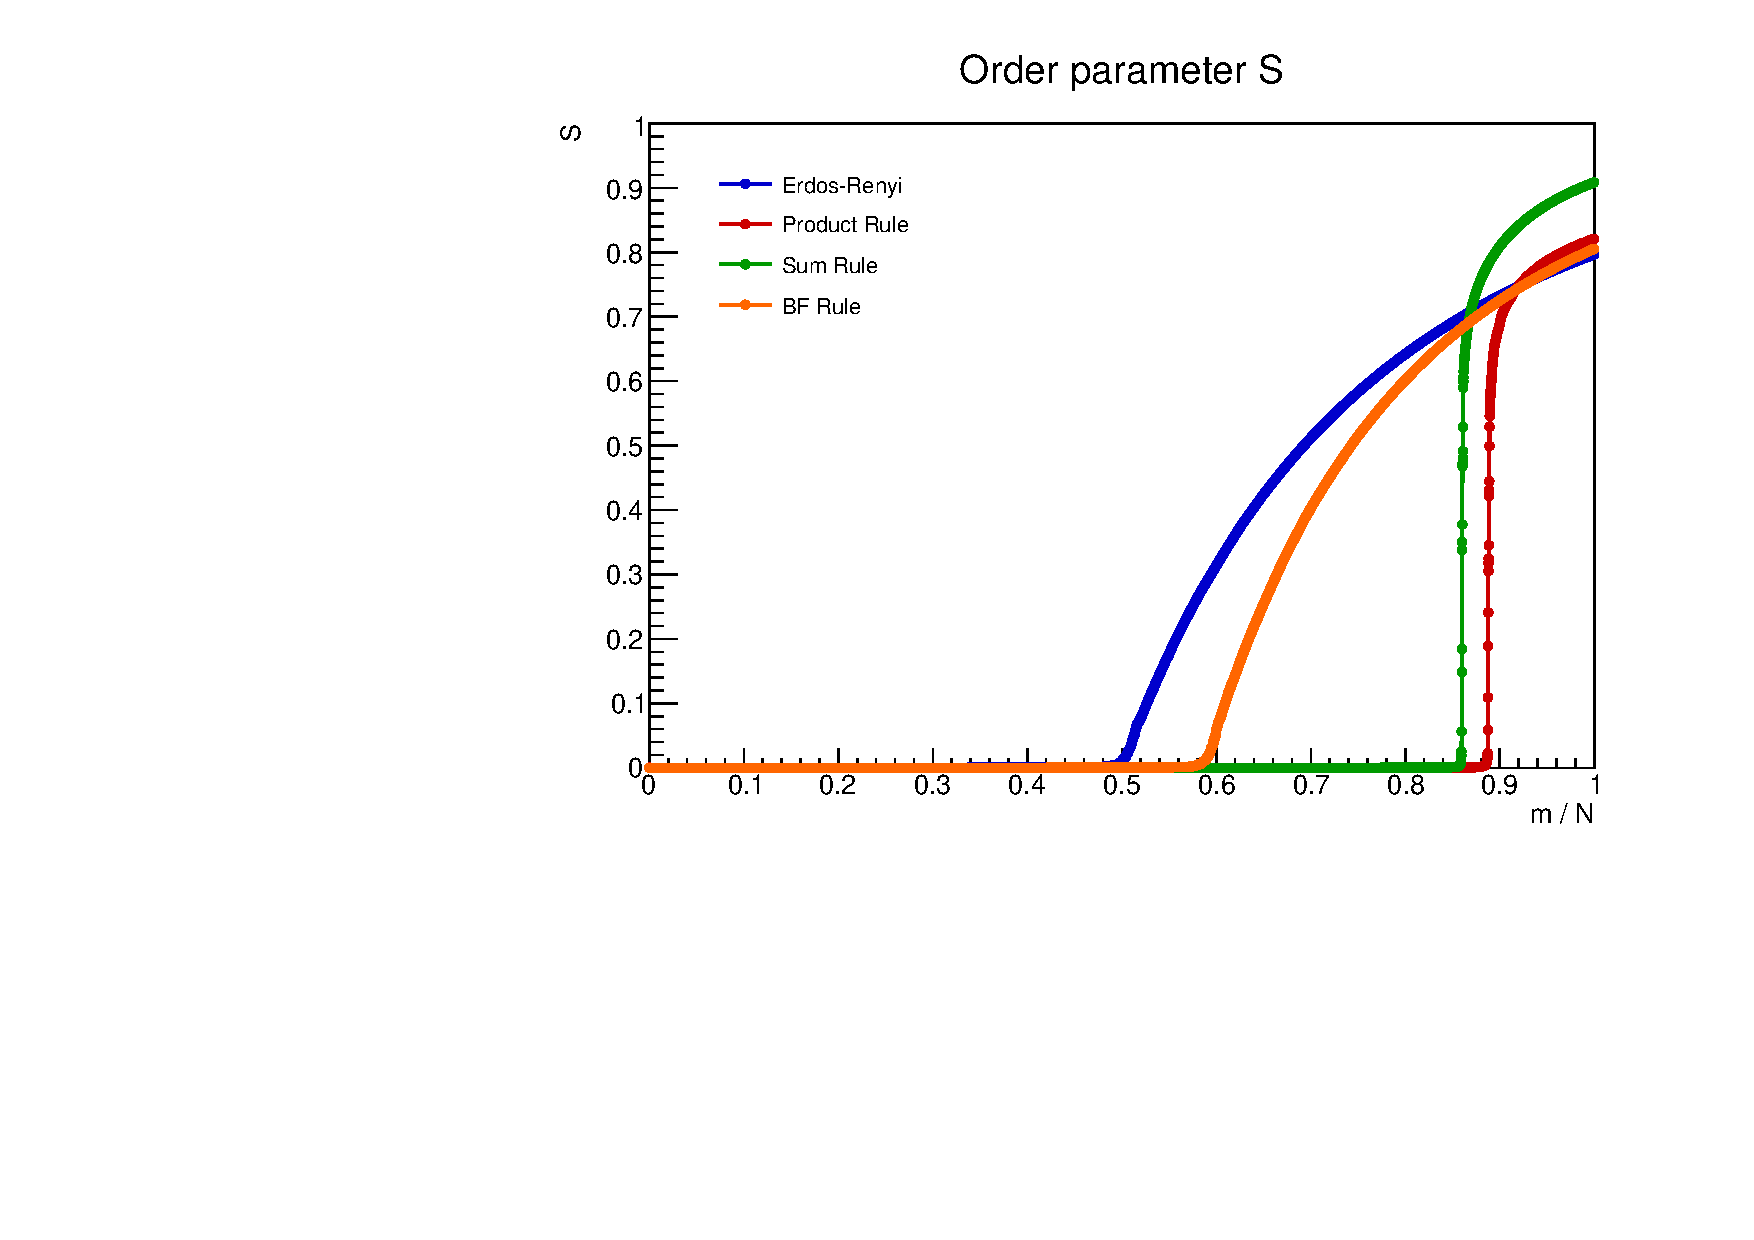
\includegraphics[width=\linewidth]{images/S.pdf}
		\caption{LCC size vs.\ added edges $m/N$, $N = 10^6$. Both ER and BF protocol give rise to a continuous phase transition, while competitive rule like PR and SR generates a seemingly looking discontinuous p.t.}
		\label{fig::S}
	\end{subfigure}
	\hspace{3pt}
	\begin{subfigure}[t]{0.48\linewidth}
		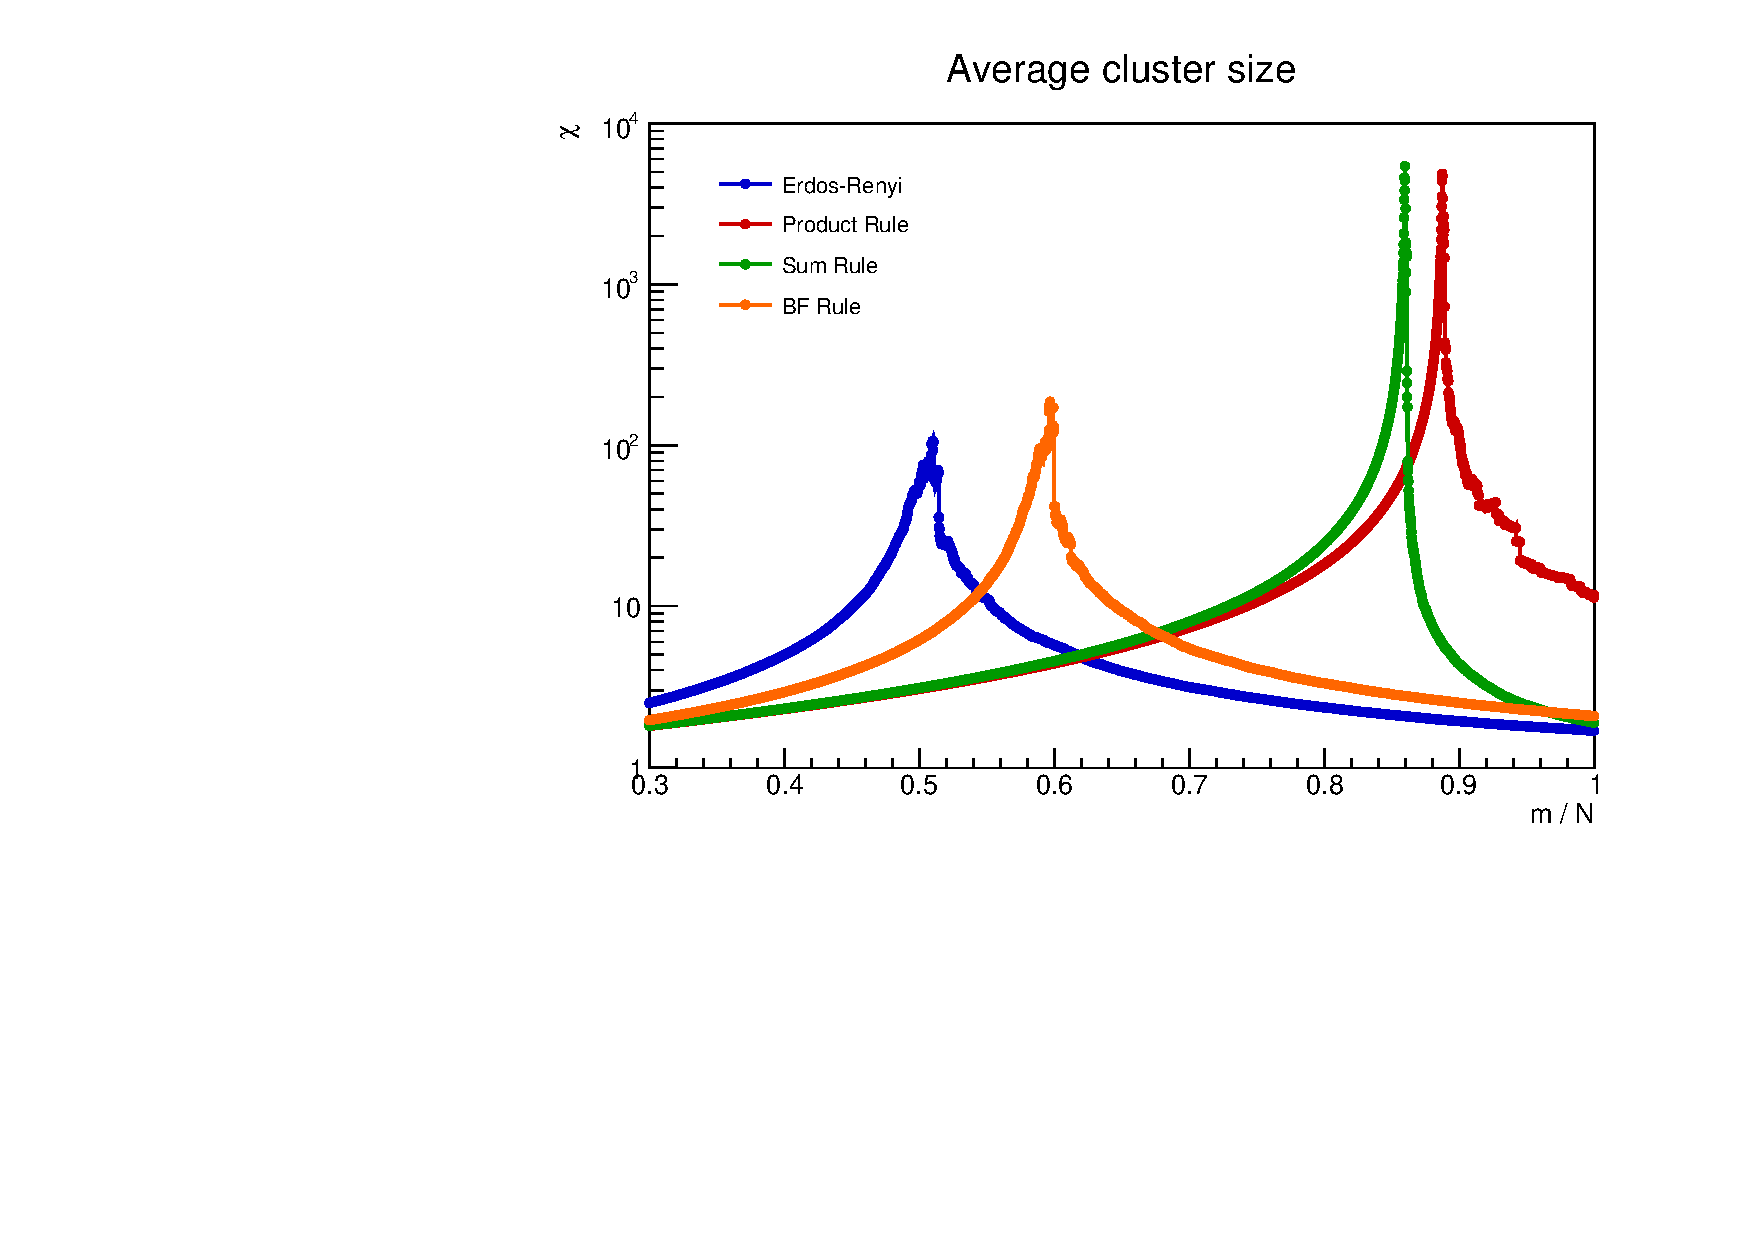
\includegraphics[width=\linewidth]{images/ACS.pdf}
		\caption{Average cluster size vs.\ $m/N$, $N = 10^6$. As expected, $\chi$ peaks when $m/N$ gets closer and closer to the critical point. Strangely enough, this is true for all generative mechanisms}
		\label{fig::ACS}
	\end{subfigure}
\end{figure}

\begin{figure}
	\centering
	\begin{subfigure}[b]{0.45\linewidth}
		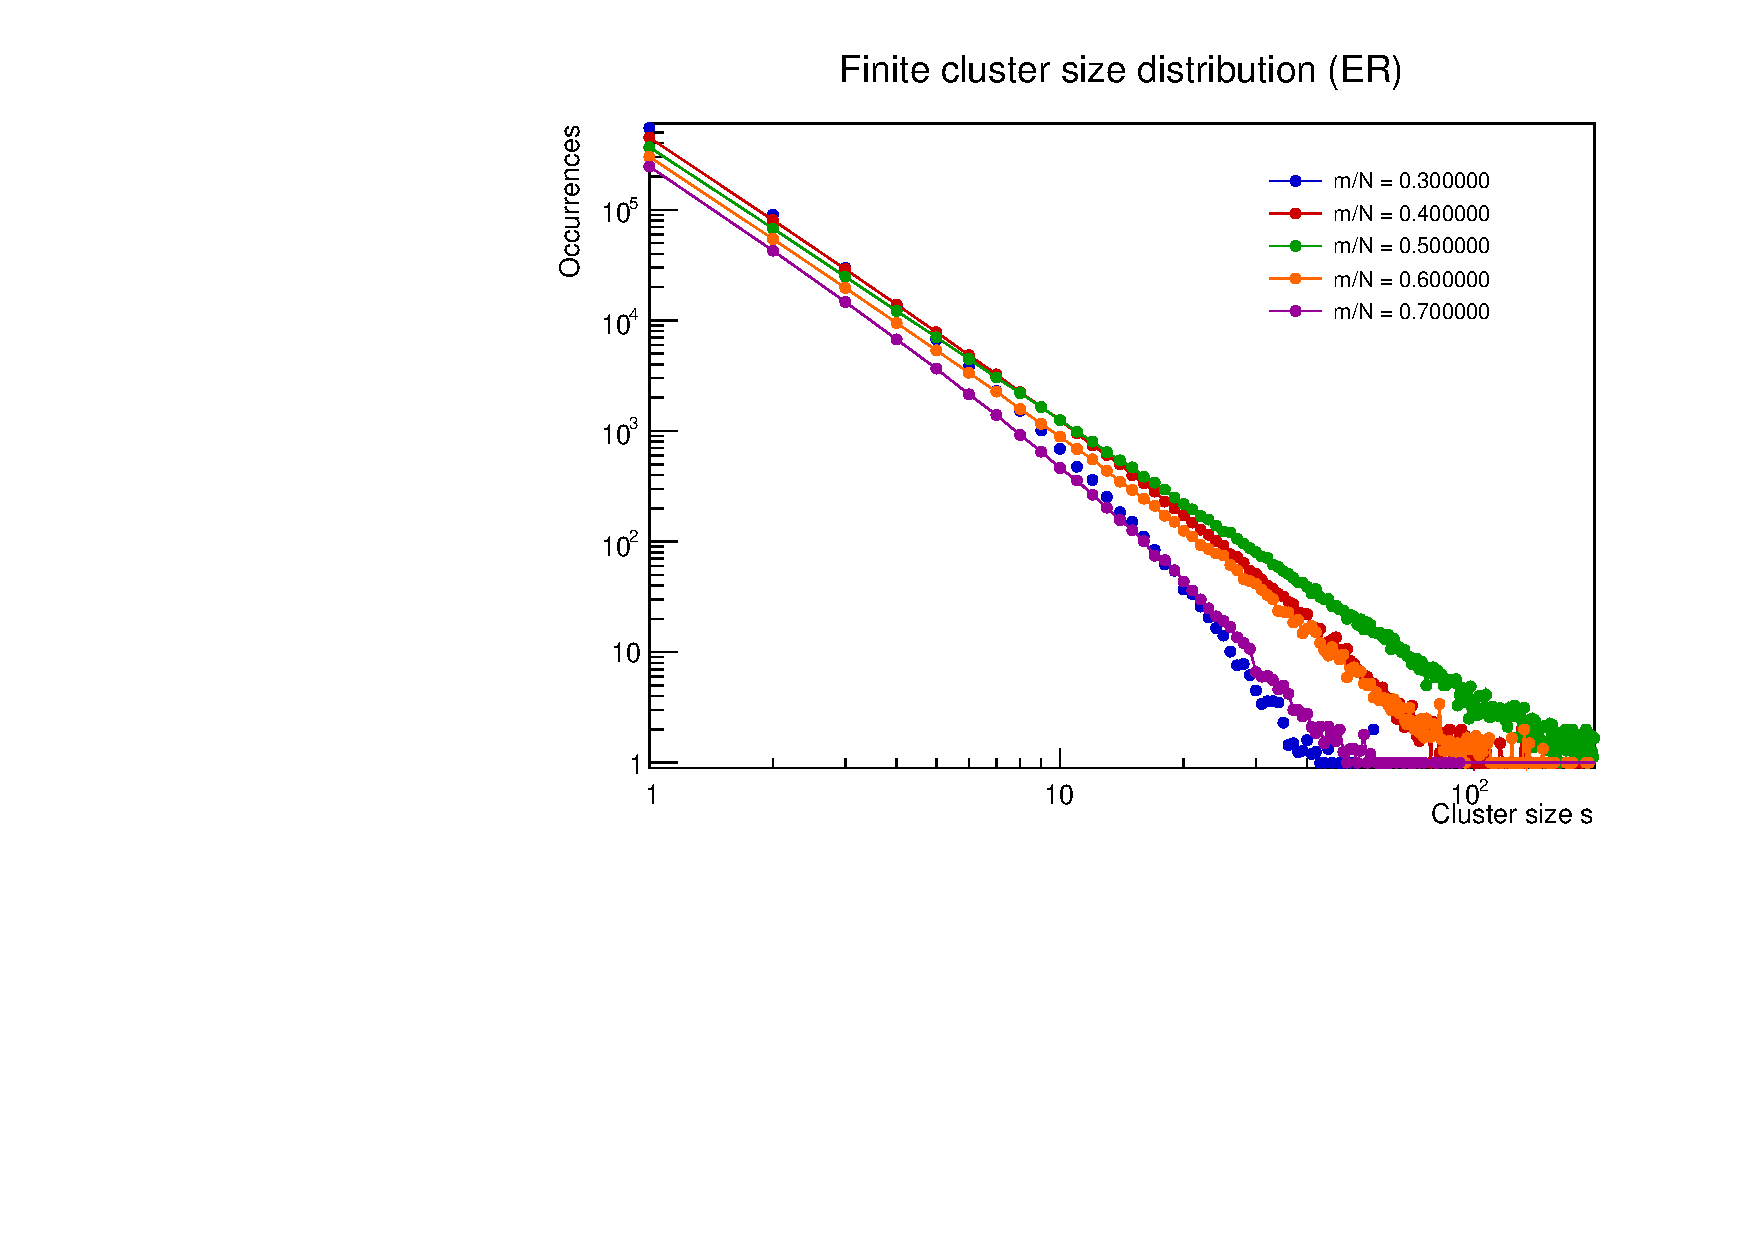
\includegraphics[width=\linewidth]{images/ClusterDistrER.pdf}
	\end{subfigure}
	\hspace{0.5em}
	\begin{subfigure}[b]{0.45\linewidth}
		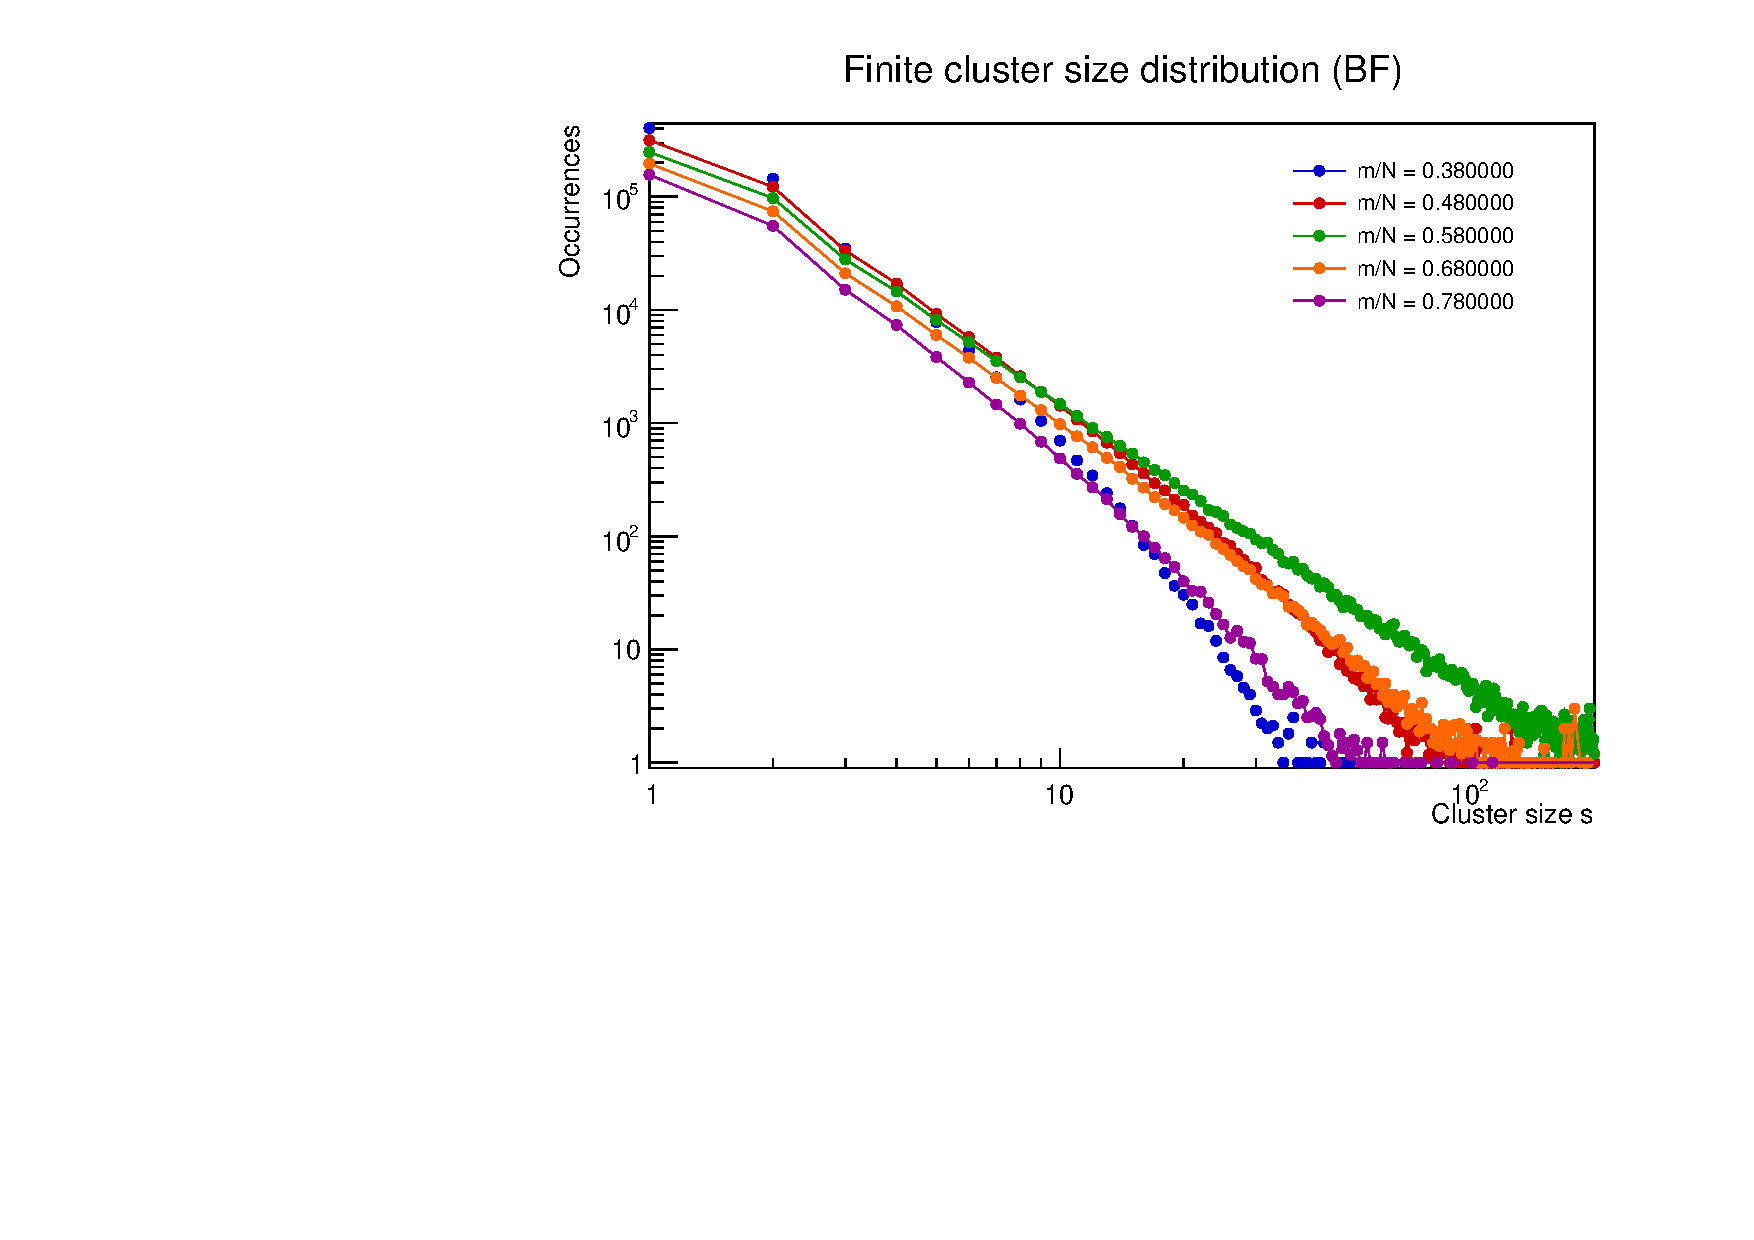
\includegraphics[width=\linewidth]{images/ClusterDistrBF.pdf}
	\end{subfigure}
	
	\vspace{0.5em} % Spazio tra righe
	
	\begin{subfigure}[b]{0.45\linewidth}
		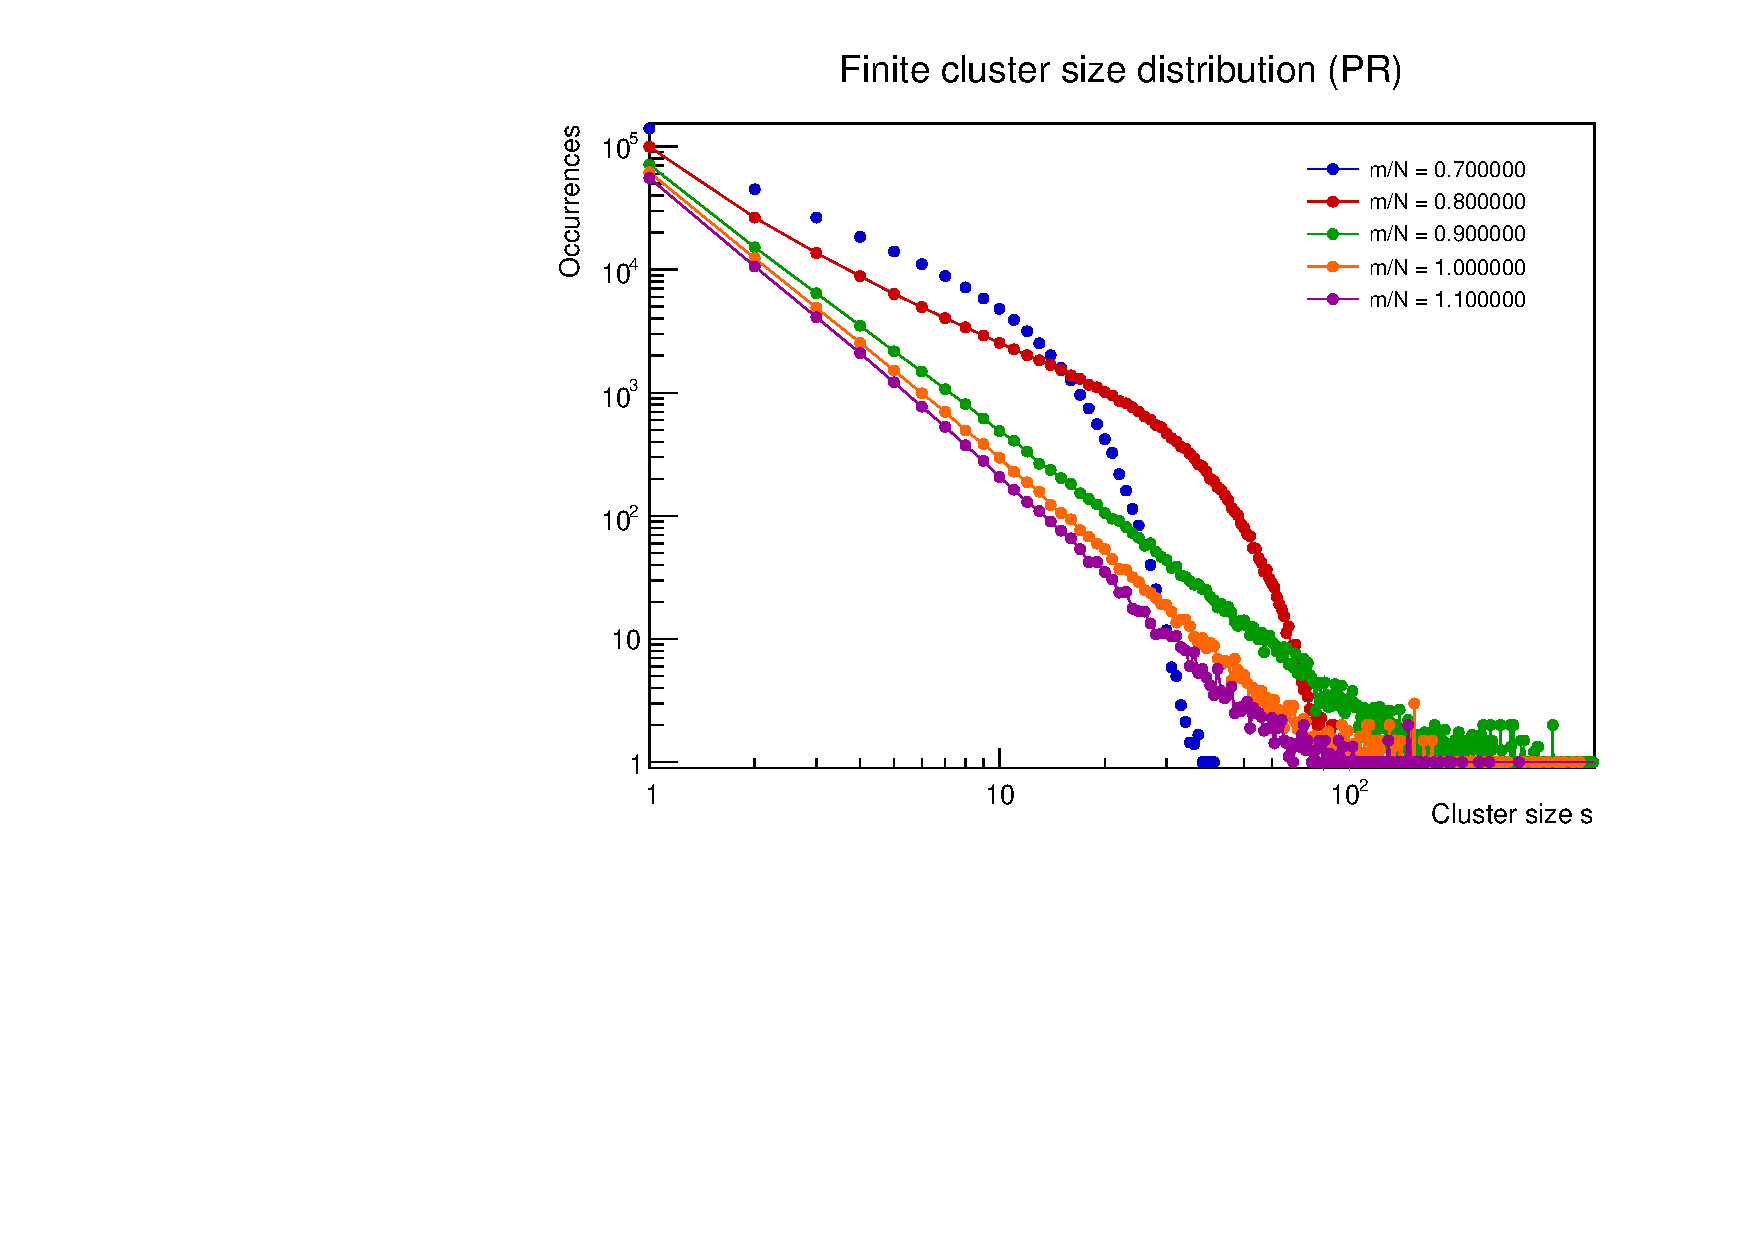
\includegraphics[width=\linewidth]{images/ClusterDistrPR.pdf}
	\end{subfigure}
	\hspace{0.5em}
	\begin{subfigure}[b]{0.45\linewidth}
		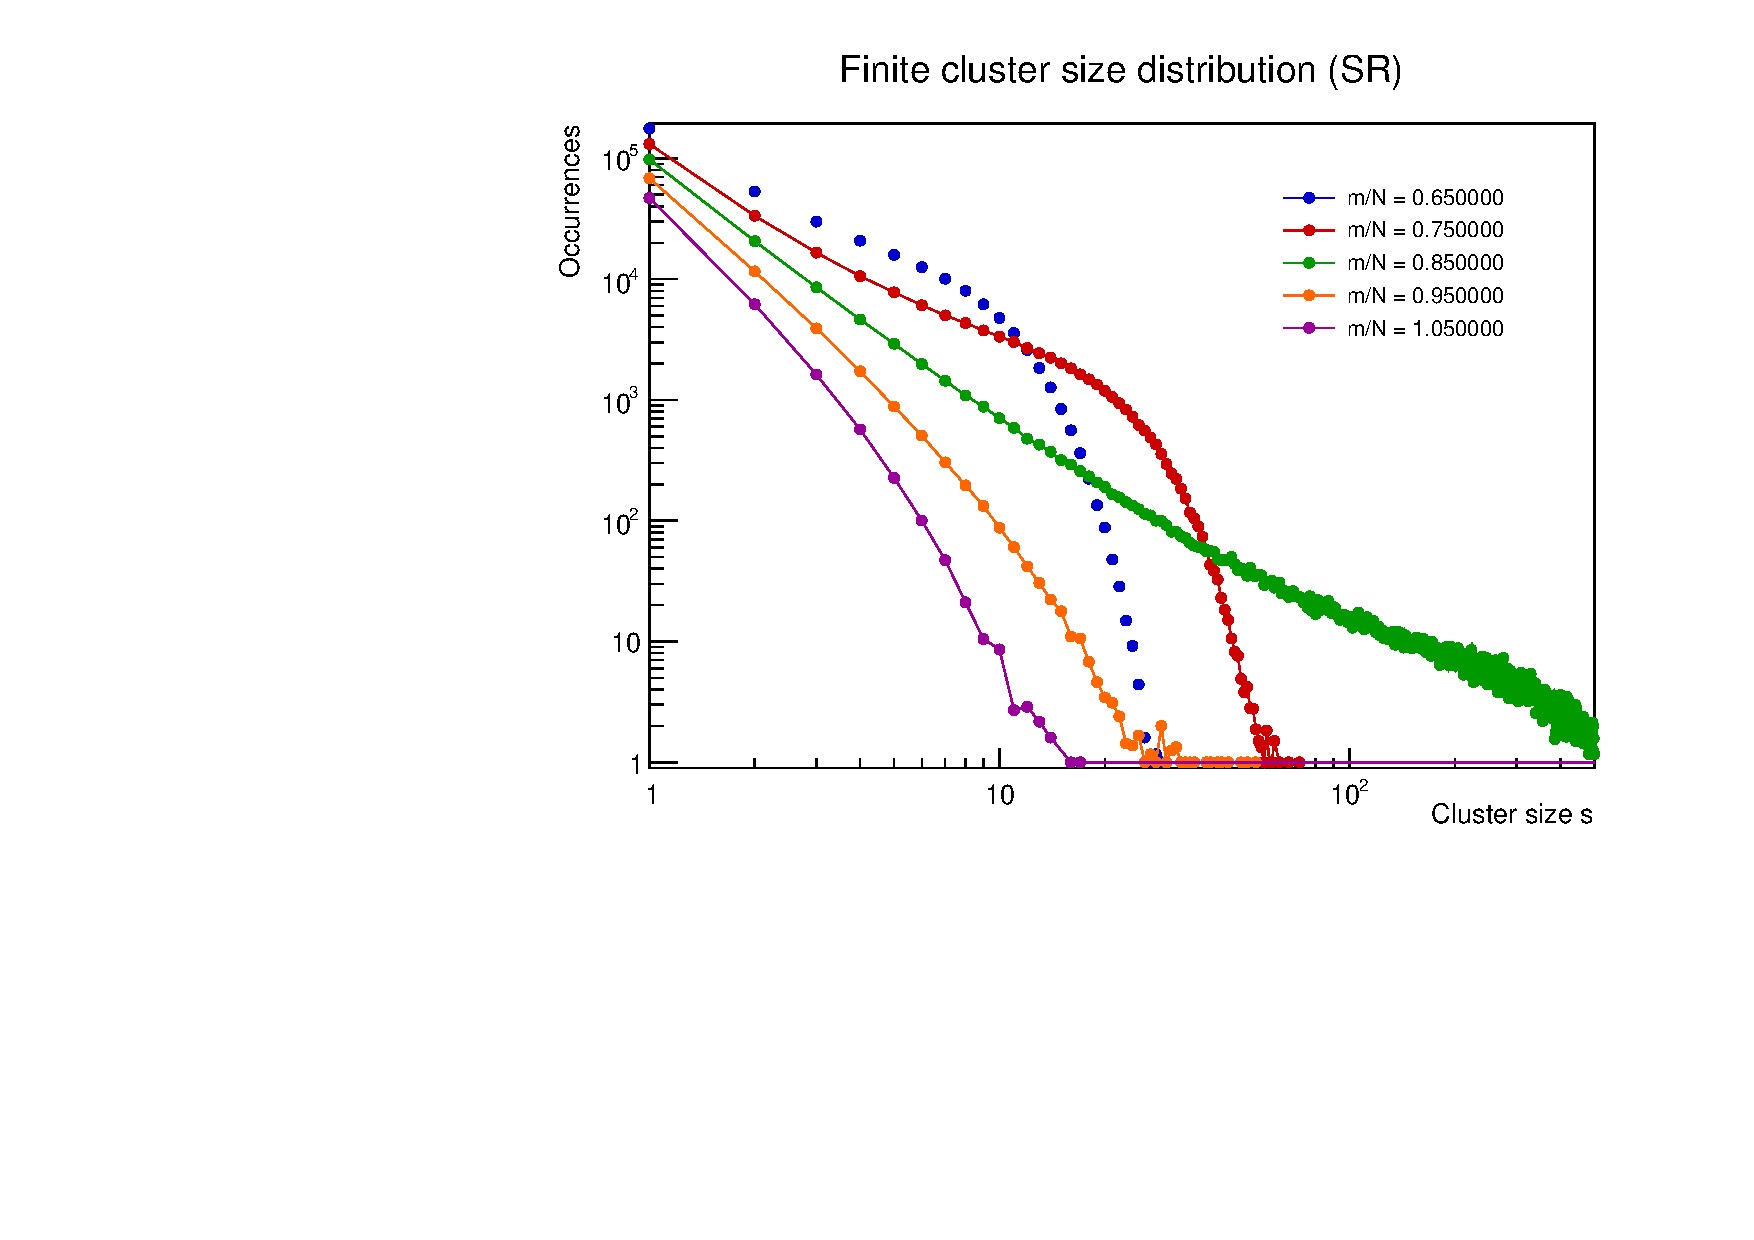
\includegraphics[width=\linewidth]{images/ClusterDistrSR.pdf}
	\end{subfigure}
	\caption{Finite cluster size distribution at and around criticality. As expected, when $m \approx m_c$, the distribution appears approximately as a power law}
	\label{fig:ClusterDistr}
\end{figure}
\section{Explosive percolation in SF networks}
We now turn our attention to a different network topology, i.e. scale-free networks whose degree distribution $P(k) \sim k^{-\gamma}$, using a configuration model. We proceed as illustrated in \cite{bibid}. Let $N$ be the initial number of totally disconnected nodes. Sampling from a power law, we associate to each node a fixed amount of stubs and we gradually proceed to connect stubs following either PR rule either a random choice (of course, when connecting stubs at random we fall back on the classical percolation problem on scale-free networks). Results for $S$ are shown in Fig \ref{fig::RGSF}, \ref{fig::PRSF}. When performing a random connection between stubs, one should expect to see a critical behaviour only when $\gamma > 3$, since $\kappa \to \infty$ for $\gamma < 3$. In fact, when $\gamma < 3$, the order parameter smoothly increases and is $0$ only when $m = 0$. When using PR rule, we observe again the abrupt change when $m \approx m_c$ together with a strange stair-like behaviour that I cannot fully explain. The most interesting result is, however, that for $\gamma = 2.6 < 3$ a phase transition is now observed. In fact, one can show \cite{bibid} that, when using PR, the threshold below which a giant cluster is always observed is $\gamma \approx 2.4$.

\begin{figure}
	\centering
	\begin{subfigure}[t]{0.48\linewidth}
		\includegraphics[width=\linewidth]{images/S_SF.pdf}
		\caption{\textit{LCC size vs.\ added edges $m/N$, $N = 10^6$, randomly connecting stubs until a power law is reached (classical percolation on SF networks)}}
		\label{fig::RGSF}
	\end{subfigure}
	\hspace{3pt}
	\begin{subfigure}[t]{0.48\linewidth}
		\includegraphics[width=\linewidth]{images/S_PR.pdf}
		\caption{\textit{LCC size vs.\ added edges $m/N$, $N = 10^6$, using PR rule to connect stubs.} }
		\label{fig::PRSF}
	\end{subfigure}
\end{figure}


\newpage